% !Mode:: "TeX:UTF-8"
%!TEX program  = xelatex

%\documentclass{cumcmthesis}
\documentclass[withoutpreface,bwprint]{cumcmthesis} %去掉封面与编号页

\usepackage{url}
\usepackage{tikz}
\usepackage{xcolor}
\usepackage{graphicx} % 图片插入需要的宏包
\usepackage{float}
\usepackage{subcaption}
\usepackage{zhlipsum,mwe}
\usepackage{mathrsfs}
\usepackage{multirow}
\usepackage{floatrow}
\usepackage{tikz}
\usepackage{booktabs}
\usepackage{threeparttable}
\usepackage{adjustbox}
\usepackage{floatrow}
\usepackage{xcolor}
\usepackage{wrapfig}
\lstset{ 
  backgroundcolor=\color{white},   				% 选择代码背景,必须加上\usepackage{color}或\usepackage{xcolor}.
  basicstyle=\footnotesize,        				% 设置代码字号.
  breakatwhitespace=false,        				% 设置是否当且仅当在空白处自动中断.
  breaklines=true,                				% 设置自动断行.
  captionpos=b,                    				% 设置标题位置.
  commentstyle=\color{green},    				% 设置注释格式
  deletekeywords={...},           				% 是否删除给定语言的关键词.
  escapeinside={\%*}{*)},          				% 是否在代码中添加LaTex. 
  frame=single,	                   				% 给代码区添加边框.
  keepspaces=true,                 				% 保留空格(useful for keeping indentation of code (possibly needs columns=flexible).
  keywordstyle=\color[RGB]{40,40,255},          % 关键字显示风格.
  morekeywords={begin}, 			% 是否需要添加其他关键词
  numbers=none,                    				% 给代码添加行号,可取值none, left, right.
  numbersep=5pt,                   				% 设置行号与代码之间的间隔
  numberstyle=\tiny\color{gray}, 				% 行号的字号和颜色
  rulecolor=\color{black},         				% 边框颜色,如果没有设置,框架颜色可以在非黑色文本中的换行符上更改(例如 text (e.g. comments (green here)))
  showspaces=false,                				% 显示每个地方添加特定下划线的空格; 覆盖了'showtringspaces'
  showstringspaces=false,          				% 仅在字符串中允许空格
  showtabs=false,                  				% show tabs within strings adding particular underscores
  stepnumber=2,                    				% the step between two line-numbers. If it's 1, each line will be numbered
  stringstyle=\color{teal},     				% string literal style
  tabsize=2,	                   				% 将默认tab设置为2个空格
  title=\lstname,                  	 			% show the filename of files included with \lstinputlisting; also try caption instead of title
  language=Matlab
}
\usetikzlibrary{patterns}
\title{基于问卷数据的居民生活及饮食习惯分析}
\tihao{A}
\baominghao{4321}
\schoolname{华中农业大学}
\membera{余航雷}
\memberb{郑妙}
\memberc{刘晨奇}
\supervisor{侯志敏}
\yearinput{2023}
\monthinput{08}
\dayinput{14}

\begin{document}

 \maketitle
 \begin{abstract}
本文主要通过对问卷数据的处理分析,分析了居民饮食习惯的合理之处以及不足之处,并说明了主要存在的问题。通过$\text{Kendall-}\tau$系数检验说明了居民的生活习惯以及饮食习惯与年龄等因素无关,通过方差分析深入分析了常见慢性病相关联的因素及相关程度。通过随机森林算法对居民进行了合理分类。

针对问题一,本文首先对问卷数据进行预处理,剔除无效问卷并将问卷数据转换为具体数据,再根据数据特征分析了居民饮食的习惯合理性以及存在对奶类食品使用频率不达标、鱼肉蛋类摄入量偏高等问题。

针对问题二,本文首先将生活习惯数据量化为身体活动情况数据,将饮食习惯数据量化为各食物每日进食量。通过分别计算各因素与生活习惯和饮食习惯间的$\text{Kendall-}\tau$系数,认为生活习惯和饮食习惯与年龄等因素并无显著相关性。

针对问题三,在第二问生活情况及饮食情况量化基础上,通过方差分析分别计算各因素与慢性病间的$F$值,并认为常见慢性病与吸烟、饮酒、生活习惯和饮食习惯间存在显著的相关性,其中与高血压相关程度最高的因素为是否吸烟以及吸烟频率,与糖尿病相关程度最高的因素为水果食用频率以及食用量。

针对问题四,本文通过随机森林算法对居民分为四类,分类器$AUC$值最高能达到0.97,因此我们认为该分类器性能较优。对四类居民问卷数据分别分析,给出了针对各类人群有利于身体健康的膳食和运动方面的合理建议。

\keywords{$\text{Kendall-}\tau$系数\quad  方差分析\quad   随机森林算法}
\end{abstract}

%目录
\tableofcontents

















\clearpage
\section{问题重述}
\subsection{问题背景}
近年来,随着社会经济的发展和生活方式的改变,慢性病在全球范围内显著上升,成为危害人类健康的重要公共卫生问题。慢性病的发展与个体的生活方式紧密相关。生活方式因素,如饮食习惯、体育锻炼、吸烟、饮酒等,被认为在慢性病的发生和发展中扮演着重要角色。不同的饮食结构、身体活动水平和生活习惯可能对慢性病的风险产生显著影响。为了更好地理解这种关联,必须进行深入研究,以便制定更精确的预防和干预策略。

\subsection{问题重述}


健康状况与多种因素密切相关,其中包括个体的年龄、饮食习惯、身体活动水平、职业等。为了探究如何通过科学的方法来提升个体的身体健康水平,合理的膳食、适度的身体运动以及践行健康的生活方式成为了社会关注的焦点,我们需要分析慢性病患病率上升的原因,并通过调查问卷数据以及营养学准则,探讨慢性病与居民饮食习惯、生活习惯等因素之间的关系。同时,我们将基于附件A2中的具体数据情况,提出针对不同人群的身体健康建议。

问题一要求我们根据附件A3中所给居民膳食指南分析附件A2中被调查者的饮食习惯合理与否,并对存在的主要问题加以分析。

问题二要求我们分析居民的生活习惯以及饮食习惯是否与年龄、性别等因素存在相关性并加以说明。

问题三要求我们根据附件A2中的数据分析慢性病与吸烟、饮酒、饮食习惯等因素的相关性以及相关程度。

问题四要求我们根据附件A2中的数据对居民进行分类,并且对每一类人群提出有利于身体健康的针对性建议。
\section{模型假设}

\begin{itemize}
\item 我们一个月按照30天或者4周来计算
\item 我们认为调查问卷的为真实填写,即问卷信度达标
\item 我们认为居民膳食指南对所有居民适用,并不存在特殊不适用人群
\end{itemize}

\section{符号说明}
\begin{table}[H]
  \centering
  \begin{tabular}{p{60pt}<{\centering}|p{60pt}<{\centering}p{180pt}<{\raggedright}}
   \hline
    序号 & 符号 & 符号说明 \\
   \hline
    1 & $n_{i+}$&第$i$行观测值数\\
    2&$n_{+j}$&第$j$列观测值数\\
    3&$n_{ij}$&第$i$行第$j$列的观测值\\
    4&$n_{++}$&表示观测值总数 \\
    \hline
  \end{tabular}
  %\caption{符号与说明}
  \label{symbol}
\end{table}
\section{问题分析}

\subsection{问题一分析}
对于问题一,我们需要对问卷数据进行处理,包括缺失值和异常数据的处理,无效问卷的剔除以及问卷数据的整合。接下来我们对问卷饮食习惯数据处理为:平均每月食用次数,平均每天食用量等以满足问题求解要求,接下来对数据进行处理分析,对照附件A2居民膳食指南分析居民饮食习惯是否合理,并指出主要存在的问题。
\subsection{问题二分析}
对于问题二,我们需要将生活习惯和饮食习惯量化为具体指标,例如吸烟情况量化为每天/支以及被动吸烟的平均天数,由于年龄为连续变量,性别、婚姻状况等为分类变量,我们需要分别建立模型进行求解。对于连续变量,我们首先对年龄进行排序,再通过计算Spearman等级相关系数分析年龄与生活习惯以及饮食习惯间相关性。对于性别和婚姻状况,我们可以计算其点双列秩相关系数(Point-Biserial Correlation Coefficient)进行相关性分析。文化程度和职业因素为多分类变量,我们通过计算其$\text{Kendall-}\tau$相关系数判断其相关性。
\subsection{问题三分析}
对于问题三,我们慢性病的问卷数据量化为是否存在该疾病,由此可见相关性为一个变量为二分类一个变量为连续变量情况,我们通过方差分析(ANOVA)判断其相关性及相关程度,并列出与慢性病相关因素及其相关程度。
\subsection{问题四分析}
对于问题四,我们需要对居民进行合理分类,各居民问卷数据具有高维数据和复杂的数据结构特征,经过处理后缺失值填补为平均值,我们可以采用常见的分类学习算法例如随机森林(Random Forest)和支持向量机(Support Vector Machines,SVM)对居民进行分类,并提取各分类中居民的饮食情况和运动情况数据分别进行分析,对每类居民提出合理的建议。
\section{问题一求解}
本题数据为问卷数据,对于问卷数据的处理包括数据资料的整理和数据资料的分析。

我们首先对异常问卷数据进行处理。对于一些可能由于填写错误引起的问卷异常,我们选择保留该项数据。例如问题D1-D3中一周吃早/中/晚餐和不吃早/中/晚餐天数加起来超过7天,这与事实不符,我们选择调整其不吃的天数使其符合事实。在问题D4-D30中,对于填写了b选项食用频率而a选项选择不食用该项食物的问卷,我们选择将其a选项是否食用更正为食用。对于一些无效问卷未完成的问卷、随意填答等问卷,我们可以将其视为无效问卷,进行删除该问卷数据处理。在问题D31-D37中,由于数据量较大我们认为数据符合正太分布,选择用$3\sigma$原则对离群问卷数据进行删除处理,对于问卷中的缺失数据,我们选择用该项数据的平均值进行填充。

接下来我们将数据处理为各食物每月的食用频率以及食用量,我们就可以得到各食物平均食用频率、食用人数占比以及平均每月食用量。结果见表\ref{1}:
\begin{table}[!ht]
\centering
\caption{饮食习惯数据}
\label{1}\resizebox{\textwidth}{!}{
\begin{tabular}{ccccc}
\hline
食物编号 & 食物类型             & 平均食用频率(次/月) & 食用人数占比(\%)  & 平均每天食用量(g)  \\ \hline
D4   & 大米               & 60.8219755  & 99.2215416  & 106.978332  \\
D5   & 小麦面粉             & 10.60548749 & 82.36345074 & 96.1044876  \\
D6   & 杂粮(小米/高粱/玉米/红豆等) & 4.947026544 & 77.71822358 & 86.82923211 \\
D7   & 薯类(红薯/山药芋头/土豆等)  & 4.809290454 & 84.44359367 & 56.49160422 \\
D8   & 油炸面食(油条/油饼等)     & 1.449489535 & 34.4691169  & 73.82573823 \\
D9   & 猪肉               & 41.99226646 & 98.07299643 & 80.25228733 \\
D10  & 牛、羊肉             & 3.287149056 & 68.89994895 & 87.11473284 \\
D11  & 禽肉               & 7.458154671 & 93.72128637 & 110.625431  \\
D12  & 内脏类              & 2.157771822 & 55.57682491 & 67.08697799 \\
D13  & 水产品              & 13.21064319 & 94.55079122 & 117.222545  \\
D14  & 鲜奶               & 7.251237876 & 53.67534456 & 228.2813746 \\
D15  & 奶粉               & 1.089497192 & 8.843797856 & 25.09025102 \\
D16  & 酸奶               & 5.205985197 & 49.56610516 & 198.5220289 \\
D17  & 蛋类               & 12.5110388  & 95.67381317 & 67.96986837 \\
D18  & 豆腐               & 7.233958652 & 92.02399183 & 96.56758454 \\
D19  & 豆腐丝/千张/豆腐干       & 2.487059724 & 48.45584482 & 76.7511263  \\
D20  & 豆浆               & 7.50553854  & 74.24706483 & 194.3994906 \\
D21  & 干豆类(黄豆/黑豆/青豆)    & 3.493797856 & 64.98213374 & 70.35392331 \\
D22  & 新鲜蔬菜             & 55.61294028 & 98.67279224 & 156.1687009 \\
D23  & 海带、紫菜等海草类        & 3.693300153 & 77.75650842 & 62.62388263 \\
D24  & 咸菜               & 3.685528331 & 62.697805   & 43.25351803 \\
D25  & 泡菜               & 1.210056151 & 25.45941807 & 41.60947058 \\
D26  & 酸菜               & 1.875816743 & 46.60541092 & 50.44473056 \\
D27  & 糕点               & 5.449042879 & 72.91985707 & 89.21277463 \\
D28  & 新鲜水果             & 26.70179939 & 97.67738642 & 167.4840718 \\
D29  & 果汁饮料             & 5.13140633  & 56.68708525 & 327.5441622 \\
D30  & 其他饮料             & 5.20086779  & 47.52424706 & 376.3493154 \\ \hline
\end{tabular}}
\end{table}

从表格中可以看出,居民以大米为主食,食用人数占比达到99.2\%,每天食用的膳食基本包括了谷薯类、蔬菜水果、禽畜鱼蛋和豆类食物。摄入食物种类也能够保证一天12种以上。居民对奶类食用频率不达标,平均食用频率13.5次/月,平均每天食用量为451.9g,由此可见应当适量提高奶制品使用频率。居民平均每天摄入蔬菜的量仅有156.1g,新鲜水果摄入量也仅达到161.5g,略低于每天应摄入量,居民应提高新鲜蔬菜水果的摄入量。居民每周摄入水产品和鸡蛋的频率和摄入量达标,鱼禽、蛋类和禽肉的平均摄入量达到295.9g,高于正常摄入水平,应减少鱼肉蛋类的摄入量。

平衡居民膳食的八条准则中提出要培养清淡的饮食习惯,由表\ref{1}可知,居民们对高盐食品,如咸菜、泡菜、酸菜等的每月食用量平均为12.9两,食用频率和食用人数占比则以咸菜居多,可达62.7\%。油炸面食的食用人数占比达到了34.5\%,平均每月食用量将近2两。高糖类食品的摄入更是难以控制,糕点类、新鲜水果、各种饮料的食用人数占比和食用量都是一个不小的数字。居民们不合理的饮食习惯体现在平日不清淡的饮食中。

各种饮料的每月摄入量可达7杯,饮料的过多摄入会对人体健康产生极大的不良影响,包括体重增加、消耗维生素等矿物质、增加患肾脏疾病的风险,甚至还可能导致骨质疏松症等。因此,居民在饮食习惯上应当有节制,尽量减少对含糖饮料和果汁类饮料的摄入,以免对自身的健康造成不良的影响。

 准则中要求成人每天摄入的油量为25~30g,由附件中所给数据进行转换,由于问卷中的食用油量调查单位为斤/月,换算可得一个月的食用量应该置于1.5~1.8斤之间才算符合标准。通过excel表格进行筛选可得出符合标准的居民数量仅有66个,占全部调查人数的0.86\%。由图\ref{t11}可知,绝大部分居民对于少油这一健康的膳食准则并未很好的执行,仍然有过多摄入烹调油这一不合理的饮食习惯。

 健康的饮食习惯应当尽量减少调味料的摄入,由所给数据可得,几乎所有的居民都食用调味料。平衡居民膳食的准则中提出了居民们每天的食用盐用量应该少于5g,附件所给数据为每月平均用量,经过换算可得一个月的食用量应该小于3两才是健康的用量。同样通过excel表格进行筛选,可以得出符合标准的居民数量只有604个,占全部调查数量的7.8\%。由此可知,绝大多数居民仍然无法控制使用食盐的用量,仍然存在着过多摄入食盐这一饮食习惯方面的问题。健康的饮食习惯应当尽量减少调味料的摄入,由所给数据可得,几乎所有的居民都食用调味料。平衡居民膳食的准则中提出了居民们每天的食用盐用量应该少于5g,附件所给数据为每月平均用量,经过换算可得一个月的食用量应该小于3两才是健康的用量。同样通过excel表格进行筛选,可以得出符合标准的居民数量只有604个,占全部调查数量的7.8\%。由此可知,绝大多数居民仍然无法控制使用食盐的用量,仍然存在着过多摄入食盐这一饮食习惯方面的问题。
\begin{figure}[H]
  \centering

  \begin{subfigure}[b]{0.45\textwidth}
    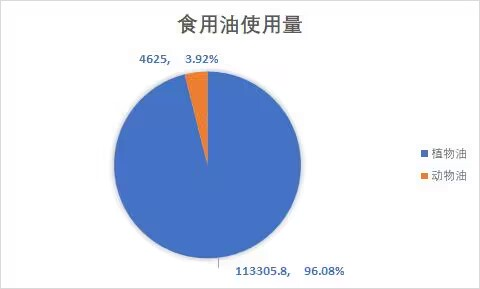
\includegraphics[width=\textwidth]{figures/QQ图片20230813183040.jpg}
    \caption{食用油使用量}
    \label{t11}
  \end{subfigure}
  \hfill
  \begin{subfigure}[b]{0.45\textwidth}
    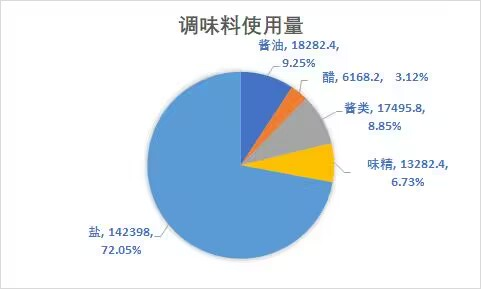
\includegraphics[width=\textwidth]{figures/QQ图片20230813170545.jpg}
    \caption{调味料使用量}
    \label{t12}
  \end{subfigure}
  \caption{食用油及调味料使用量}
\end{figure}
% 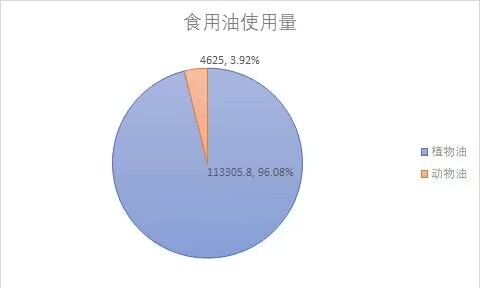
\includegraphics[width=0.4\textwidth]{figures/QQ图片20230813170116.jpg}
% 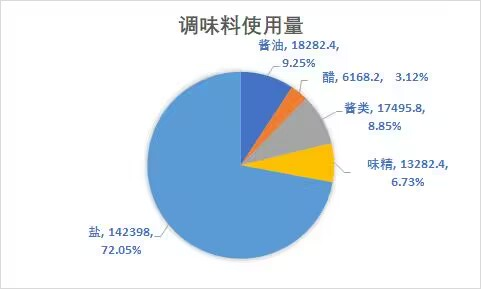
\includegraphics[width=0.4\textwidth]{figures/QQ图片20230813170545.jpg}

% \end{figure}



无论男女老少,酒精的过多摄入都是不利于健康的,由图  数据可得,仍然有很多居民饮酒,且对各类酒的平均每次饮用量也普遍较多不符合膳食准则所要求的酒精量,一部分居民仍然存在不适量饮酒的健康问题。
\clearpage
\section{问题二模型建立和求解}
要分析居民的生活习惯和饮食习惯与年龄、性别、婚姻状况、文化程度、职业等因素的相关性,我们采取$\text{Kendall-}\tau$相关系数来判定。
\subsection{$\text{Kendall}$相关性分析}
对于定类变量我们计算其$\text{Kendall-}\tau$系数度量相关性强弱,$\text{Kendall-}\tau$通过计算两个变量的所有可能观测对之间的一致对和不一致对的数量来计算,如式\ref{s1}所示:
\begin{eqnarray}
\text{Kendall-}\tau=\frac{\sum_{i<k}\sum_{j<l}n_{ij}n_{kl}-\sum_{i<k}\sum_{j>l}n_{ij}n_{kl}}{\sqrt{(\frac{n_{++}(n_{++}-1)}{2}-\frac{\sum_in_{i+}(n_{i+}-1)}{2})(\frac{n_{++}(n_{++}-1)}{2}-\frac{\sum_jn_{+j}(n_{+j}-1)}{2}})}\label{s1}
\end{eqnarray}
其中,$n_{i+}$表示第$i$行观测值数,$n_{+j}$表示第$j$列观测值数,$n_{ij}$表示第$i$行第$j$列的观测值,$n_{++}$表示观测值总数。

我们通过计算得到年龄、性别、婚姻状况、文化程度、职业等因素与生活习惯与饮食习惯的$\text{Kendall-}\tau$系数,结果见图\ref{2}:
\begin{figure}[H]
\centering
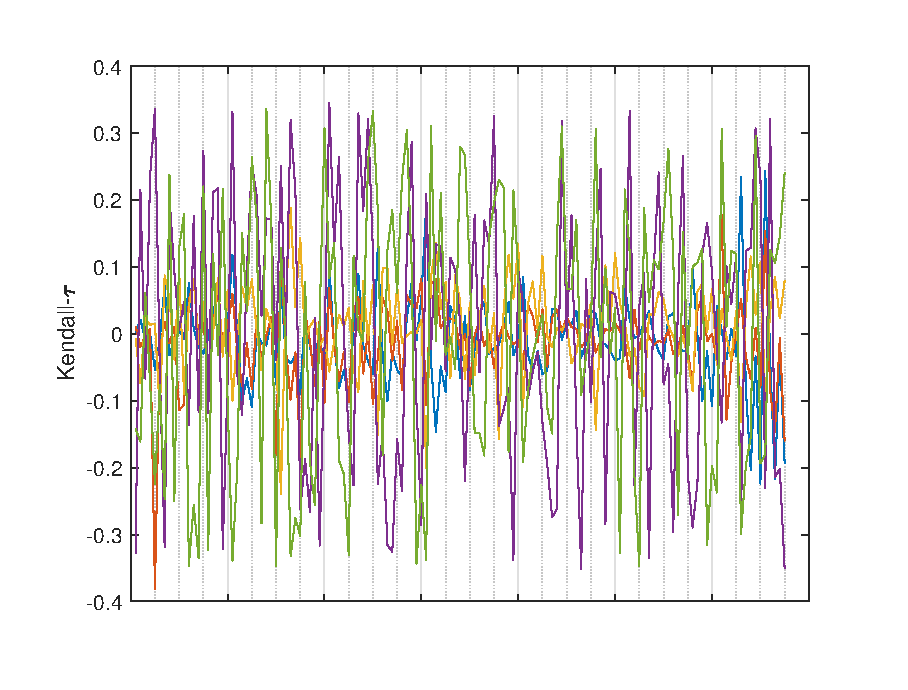
\includegraphics{figures/A2.eps}
\caption{$\text{Kendall-}\tau$系数}\label{2}
\end{figure}

以性别和饮食习惯为例,我们将$\text{Kendall-}\tau$系数从高到低排序并绘制如图\ref{3}所示。我们发现${Kendall-}\tau$相关系数绝对值均不超过0.3,我们认为不存在显著相关性。
\begin{figure}[H]
\centering
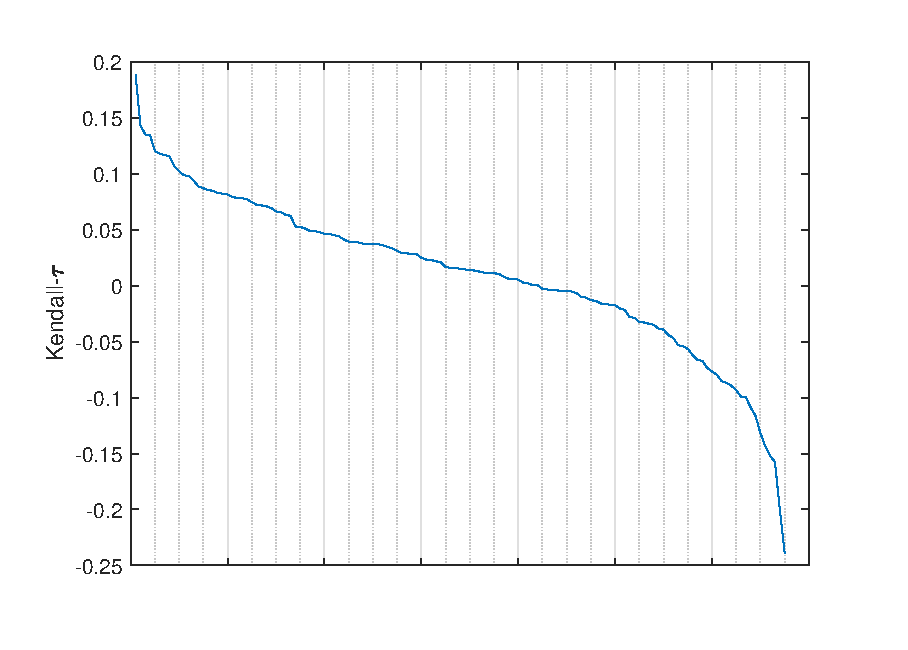
\includegraphics{figures/A1.eps}
\caption{性别与饮食习惯的$\text{Kendall-}\tau$系数}\label{3}
\end{figure}
\clearpage
\section{问题三模型建立与求解}
对于高血压和糖尿病的影响因素分析,在问卷数据中高血压和糖尿病为二分类变量,我们采用方差分析法寻找该慢性病的影响因素以及相关程度。
\subsection{ANOVA介绍}
方差分析(ANOVA,Analysis of Variance)是一种用于比较不同组之间均值差异是否显著的统计方法。它将总体方差分解为组间方差和组内方差,以便评估组间差异相对于随机误差的显著性。该分析方法步骤如下:

首先我们确立原假设$H_0$:两因素间没有显著相关性以及备择假设$H_1$:两因素间存在显著相关性。

计算组内偏差$SS_e$和组间偏差$SS_A$:

\begin{eqnarray}
SS_e=\sum_{i=1}^k\sum_{j=1}^{n_i}(Y_{ij}-\bar{Y_i})^2
\end{eqnarray}

\begin{eqnarray}
SS_A=\sum_{i=1}^kn_i(\bar{Y_i}-\bar{Y})^2
\end{eqnarray}

其中,$\bar{Y}=\frac{1}{n}\sum_{i=1}^{k}\sum_{j=1}^{n_i}Y_{ij},n=n_1+n_2+\cdots+n_k$,则总偏差平方和$SS$可以表示为组内偏差和组间偏差和,计算如下:

\begin{eqnarray}
SS=SS_e+SS_A=\sum_{i=1}^k\sum_{j=1}^{n_i}(Y_{ij}-\bar{Y})^2
\end{eqnarray}

接下来就是计算$F$值来比较组间方差与组内方差的大小,$F$计算如下:
\begin{eqnarray}
F=\frac{SS_A(n-k)}{SS_e(k-1)}
\end{eqnarray}

最后我们通过计算$p$值与显著性水平比较来确定两因素之间相关性,其中$p$值计算如下:
\begin{eqnarray}
p=P(F>F_{observed}|\text{null hypothesis})
\end{eqnarray}

其中,$F_{\text{observed}}$ 是观察到的$F$统计量,$\text{null hypothesis}$是原假设,即两因素间存在显著相关性,若$p$值小于0.05,我们接受原假设认为两因素间存在显著相关性,否则接受备择假设认为两因素间不具有显著相关性。

\subsection{问题三求解}
我们分别计算各因素与高血压、糖尿病的$p$值,相关联因素以及对应$p$值见表\ref{bbb}:在表中可以发现一些因素与慢性病存在显著相关性,$p$值越小代表相关性越强。
\begin{table}[H]
\centering
\caption{与慢性病相关因素及$p$值
}
\label{bbb}\begin{threeparttable}
\begin{tabular}{ccc}
\hline
相关因素    & 与高血压相关因素$p$值       & 与糖尿病相关因素$p$值 \\ \hline
薯类      & *0.190943929 & 0.003827177  \\
油炸面食    & *0.361442233 & 0.046705978  \\
猪肉      & 0.043642272        & 0.016092084  \\
牛羊肉     & 0.030360716        & 0.003521846  \\
禽肉      & *0.234161903 & 0.015988882  \\
内脏      & 0.041687594        & 0.011282698  \\
水产      & *0.491465833 & 9.78E-10     \\
奶粉      & 0.001416892        & 9.45E-17     \\
蛋类      & *0.398223403 & 0.018104059  \\
豆腐      & *0.202816301 & 0.000134327  \\
豆浆      & *0.193012429 & 0.031503582  \\
新鲜蔬菜    & *0.760532978 & 0.013736621  \\
泡菜      & *0.215356076  & 0.027442675  \\
酸菜      & 3.66E-11           & 2.23E-08     \\
糕点      & 0.011306996        & 2.51E-05     \\
水果      & 0.000186068        & 1.52E-19     \\
果汁饮料    & 1.56E-05           & 0.008366292  \\
吸烟      & 2.79E-07           & 0.033829592  \\
饮酒      & 0.030320435        & 0.034272381  \\
体育锻炼 & 0.001241476        & 0.002024085  \\ \hline
\end{tabular}
\begin{tablenotes}    %这行要添加, 从这开始
        \footnotesize               %这行要添加
        \item[1] 带`*'表示无显著相关性
      \end{tablenotes}            %这行要添加
    \end{threeparttable}       %这行要添加,到这里结束
\end{table}

\section{问题四模型建立与求解}
对于高维数据和复杂的数据结构特征,我们可以采用的分类学习算法如随机森林(Random Forest)对居民进行分类。
\subsection{随机森林算法}
随机森林算法(Random Forest)是基于分类回归树 CART (Classification and Regression Tree) 发展的一种集成学习模型,它由大量相互独立构建的决策树组合而成。随机森林分类算法具有极好的准确率,能够有效的运行在大数据集上,可以处理具有高维特征的样本输入。为了评估模型的性能,采用了混淆矩阵$C.M.$,ROC曲线下面积$AUC$,分别计算如下:
\begin{eqnarray}
C.M.=\begin{bmatrix}
  TP&FN \\
  FP&TN
\end{bmatrix}
\end{eqnarray}
\begin{eqnarray}
AUC=\frac{1}{2}(\frac{TP}{TP+EN}+\frac{TP}{TP+FP})
\end{eqnarray}
其中,$TP,FP,TN$和$FN$分别是真阳性,假阳性,真阴性和假阴性的数量。选取均方误差$RMSE$,平均绝对误差$MAE$,相对绝对误差$RAE$对模型进行误差评估,,分别计算如下:
\begin{eqnarray}
RMSE = \sqrt{\frac{1}{n} \sum_{i=1}^{n} (y_i - \hat{y}_i)^2}
\end{eqnarray}
\begin{eqnarray}
MAE = \frac{1}{n} \sum_{i=1}^{n} |y_i - \hat{y}_i|
\end{eqnarray}
\begin{eqnarray}
RAE = \frac{\sum_{i=1}^{n} |y_i - \hat{y}_i|}{\sum_{i=1}^{n} |y_i - \bar{y}|}
\end{eqnarray}
其中,$n$是样本数量,$y_i$是第$i$个真实值,$\hat{y_i}$是第$i$个预测值,$\bar{y}$是真实值的平均值。
\subsection{问题四求解}
我们训练后模型$ROC$曲线如下:
\begin{figure}[H]
\centering
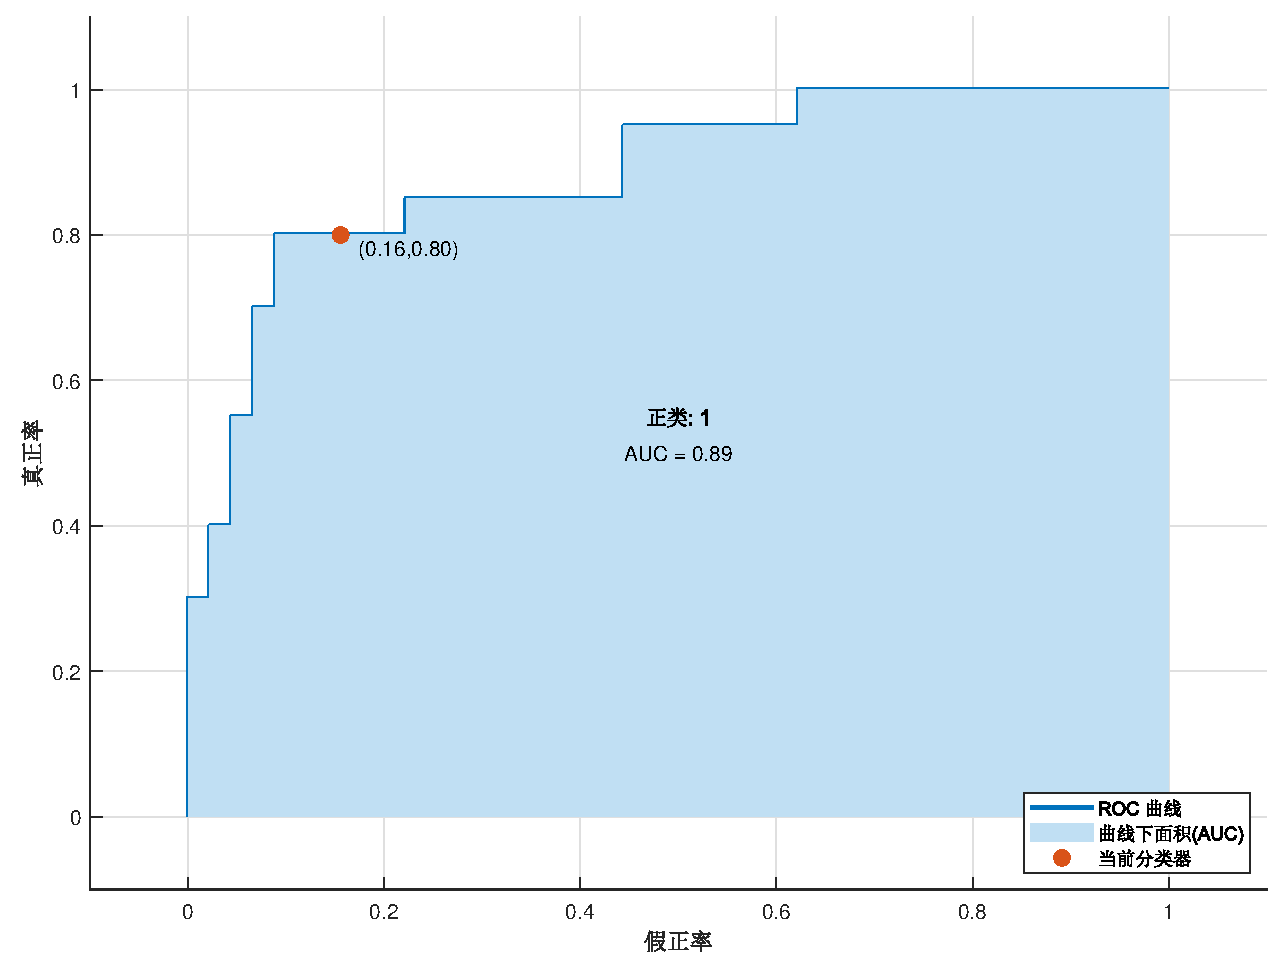
\includegraphics[width=.49\textwidth]{figures/31.eps}
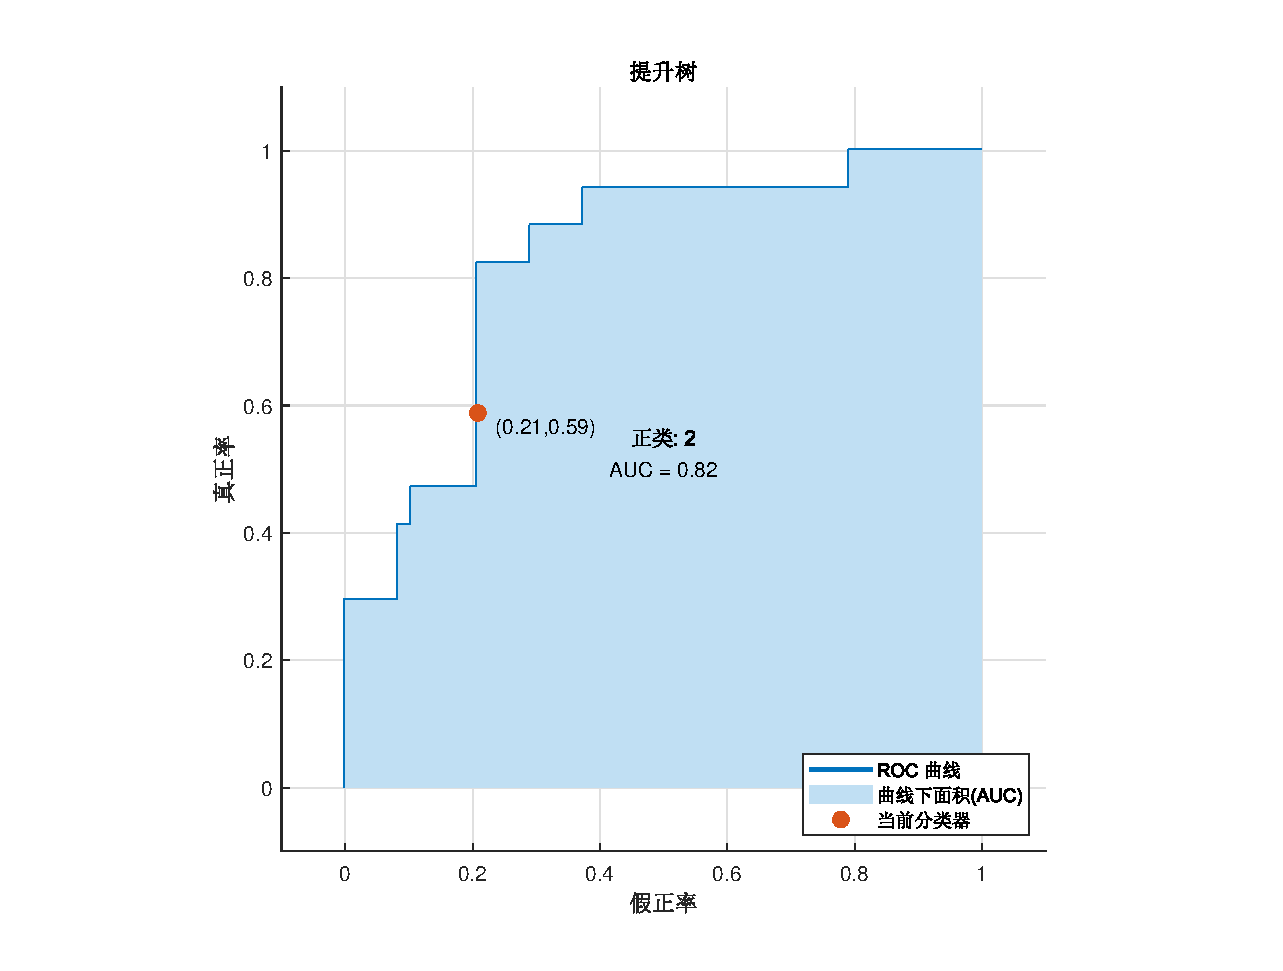
\includegraphics[width=.49\textwidth]{figures/32.eps}
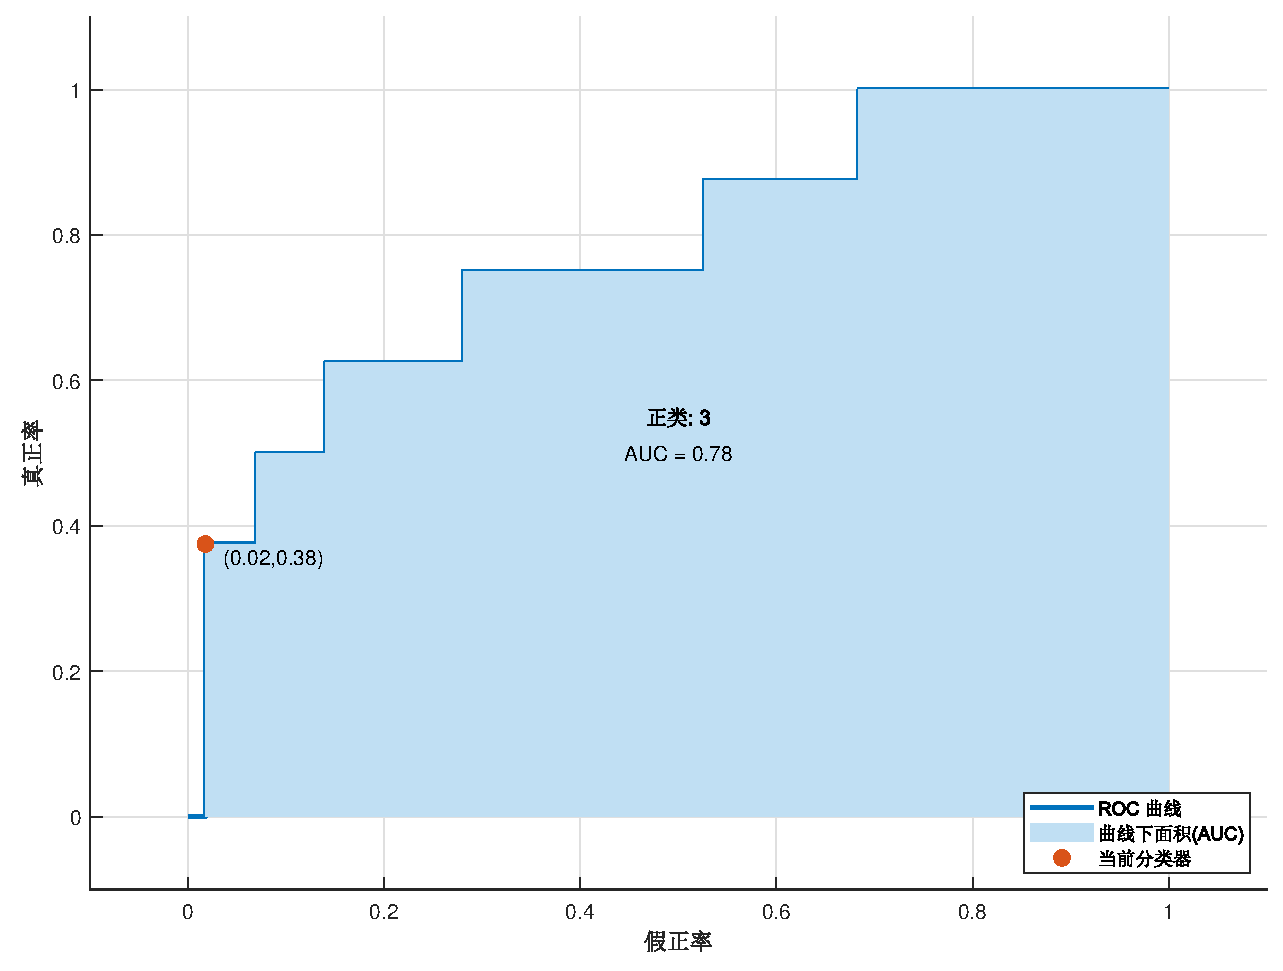
\includegraphics[width=.49\textwidth]{figures/33.eps}
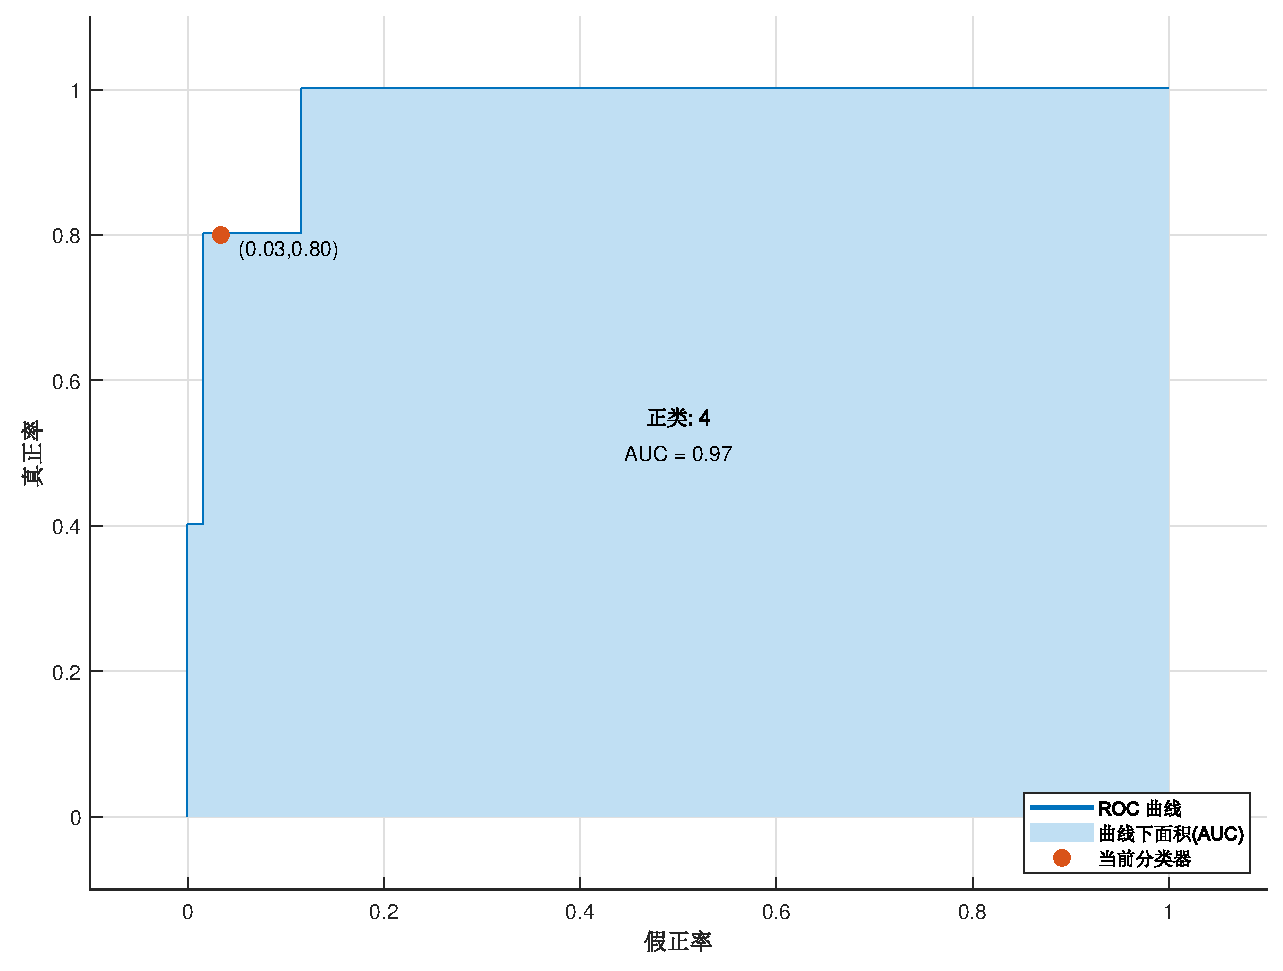
\includegraphics[width=.49\textwidth]{figures/34.eps}
\caption{测试集$ROC$曲线}
\end{figure}
我们通过机器学习将居民群体分为4大类,这四类的$AUC$值均在0.7以上,分类器准确率达到0.64,我们认为该模型分类效果良好。接下来提取每类人群的问卷数据,并分别统计分析其生活习惯及饮食习惯各项指标。我们提出以下合理意见:

第I类人群基本为未患慢性病人群,并不需要刻意控制饮食,但仍需要注意吸烟饮酒情况。第II类人群基本为患高血压人群,该类居民应当控制酸菜、吸烟等频率,增大体育锻炼的量。第III类人群为患糖尿病人群,应当根据医生要求控制糖类进食量。第VI类人群基本为某种原因未患慢性病但在血压,血糖等方面仍存在些许问题,这类居民应当即使就医,少抽烟少喝酒,增强体育锻炼等预防慢性病的发生。











%参考文献
\clearpage
\begin{thebibliography}{99}%宽度9
\bibitem{__2022}
刘世涛,  郝兵元,  杨冉, and  朱文庆.
\newblock 基于方差分析法坚硬顶板下矿压显现分析.
\newblock {\it 煤炭技术}, 41(7):20--23, 2022.
\newblock {\textless}北大核心{\textgreater}.

\bibitem{__2024}
 姚鹏飞,  涂亚楠, and  王瑞红.
\newblock 基于随机森林算法拖拉机齿轮箱故障诊断研究.
\newblock {\it 农机化研究}, 46(3):246--251, 2024.
\newblock {\textless}北大核心{\textgreater}.

\bibitem{__2013}
 孙佳韵,  方正,  程彩霞, and  王骏横.
\newblock 基于方差分析法的中庭机械排烟影响因素.
\newblock {\it 武汉大学学报(工学版)}, 46(5):640--644, 2013.
\newblock 3 citations(CNKI)[2023-8-14]{\textless}北大核心,
  CSCD{\textgreater}.

\bibitem{_anova_2021}
 张微.
\newblock
  商务翻译对跨境电子商务绩效的线性影响分析——基于{ANOVA方差分析模型的实证}.
\newblock {\it 中国产经}, (9):152--153, 2021.

\bibitem{__1989}
 朱宁波.
\newblock 问卷调查数据处理程序设计.
\newblock {\it 统计与决策}, (1):35--36, 1989.
\newblock 2 citations(CNKI)[2023-8-14].

\bibitem{_cacac_2020}
 杜华川.
\newblock {\it
  {基于试拌法和方差分析法的CA胶浆及CAC的改性研究}}.
\newblock 硕士, 汕头大学, 2020.

\bibitem{__2009}
 杨汉东.
\newblock 谈谈市场问卷调查中的数据处理.
\newblock {\em 商场现代化}, (10):164--165, 2009.
\newblock 5 citations(CNKI)[2023-8-14].

\bibitem{__2018}
 欧阳游,  梁永顺,  唐晓川,  杜晓立,  刘姗姗,  孙陶, and 
  李峰林.
\newblock 应用方差分析法检验γ测井模型的均匀性.
\newblock {\it 宇航计测技术}, 38(5):91--95, 2018.
\newblock 2 citations(CNKI)[2023-8-14]{\textless}CSCD{\textgreater}.

\bibitem{__2023}
 邓雅文, 蒋卫国 ,  王晓雅, and  彭凯锋.
\newblock
  基于随机森林算法和知识规则的国际湿地城市精细湿地分类——以常德市为例.
\newblock {\it 遥感学报}, 27(6):1426--1440, 2023.
\newblock {\textless}北大核心, EI, CSCD{\textgreater}.
\end{thebibliography}

\newpage
%附录
\begin{appendices}
\section{附件列表}
\begin{lstlisting}[language=html]
第一次培训
├─ README.md
├─ 数据.xlsx
├─ 草稿.md
├─ 第四问
│  ├─ 第四问模型
│  │  └─ wenti4.mat
│  └─ 第四问代码
│     └─ wenti4.mlx
├─ 第三问
│  └─ 代码及数据
│     ├─ A.mat
│     └─ wenti3.mlx
├─ 第一问
│  ├─ 第一问结果
│  │  └─ wenti1.mat
│  └─ 第一问数据即代码
│     ├─ 1.py
│     ├─ 2.py
│     ├─ 3.py
│     ├─ wenti1.mlx
│     └─ X.mat
├─ CUMCMThesis_2 - 副本
│  ├─ bbl.bib
│  ├─ cumcmthesis.cls
│  ├─ example.pdf
│  ├─ example.tex
│  ├─ main.tex
│  ├─ 参考手册.pdf
│  └─ figures
│     ├─ 1.png
│     ├─ 31.eps
│     ├─ 32.eps
│     ├─ 33.eps
│     ├─ 34.eps
│     ├─ A1.eps
│     ├─ A2.eps
│     ├─ gongzhonghao.jpg
│     ├─ QQ图片20230813170116.jpg
│     ├─ QQ图片20230813170545.jpg
│     └─ QQ图片20230813183040.jpg
└─ .git

\end{lstlisting}
\section{第一问MATLAB代码}
\begin{lstlisting}[language=matlab]
% 全部转化为食物次数/月,结果储存在new_X
% load('X.mat')
[num_rows, num_cols] = size(X);
new_X=zeros(num_rows,num_cols/5);
% 周期
period = 5;

% 遍历
for i = 1:period:num_cols
    % 计算新的一列数据,如果第一列为2,则结果为0,否则进行计算
    for j=1:num_rows 
        if X(j, i) == 2
            new_X(j,(i-1)/5+1)=0;
        else 
            new_X(j,(i-1)/5+1)=X(j, i+1) * 30 + X(j, i+2) * 4 + X(j, i+3);
        end
    end
end

% 各食物平均每月食用量,结果储存在nnew_X
[num_rows, num_cols] = size(X);
nnew_X=zeros(num_rows,num_cols/5);
% 周期
period = 5;

% 遍历
for i = 1:period:num_cols
    % 计算新的一列数据,如果第一列为2,则结果为0,否则进行计算
    for j=1:num_rows 
        if X(j, i) == 2
            nnew_X(j,(i-1)/5+1)=0;
        else 
            nnew_X(j,(i-1)/5+1)=(X(j, i+1) * 30 + X(j, i+2) * 4 + X(j, i+3))*X(j, i+4);
        end
    end
end

%各食物平均食用频率,结果储存在gsw_means
gsw_means = mean(new_X);
%各食物平均食用量,结果储存在ngsw_means
ngsw = mean(nnew_X);
means=[50;50;50;50;50;50;50;50;50;50;50;10;50;60;50;50;50;50;50;50;50;50;50;50;50;250;250]';
ngsw_means=zeros(size(ngsw));
for i=1:27
    ngsw_means(1,i)=ngsw(1,i)*means(1,i)/gsw_means(1,i);
end

% 各食物食用人数占比,结果储存在nonzero_percentage
[num_rows, num_cols] = size(new_X);
nonzero_percentage = zeros(1, num_cols);

% 计算每列的非零元素占比
for i = 1:num_cols
    nonzero_count = nnz(new_X(:, i)); % 计算非零元素数量
    nonzero_percentage(i) = nonzero_count / num_rows; % 计算占比
end
nonzero_percentage=100*nonzero_percentage;
\end{lstlisting}
\section{第一问PYTHON代码}
\begin{lstlisting}[language=python]
import pandas as pd
import matplotlib.pyplot as plt


csv_file_path = "data.csv"  
data = pd.read_csv(csv_file_path, encoding='GBK')


plt.rcParams['font.sans-serif'] = ['SimHei']
plt.rcParams['axes.unicode_minus'] = False 

drink_counts = data['是否饮酒'].value_counts()


labels = ['不饮酒', '饮酒', '已戒酒']
plt.figure(figsize=(8, 6))
plt.pie(drink_counts, labels=labels, autopct='%1.1f%%', startangle=140)
plt.title('饮酒情况分布')
plt.show()


drinkers_data = data[data['是否饮酒'] == 1]


average_years = drinkers_data['饮酒年数'].mean()


alcohol_columns = ['是否饮用高度白酒', '是否饮用低度白酒', '是否饮用啤酒', '是否饮用黄酒、糯米酒', '是否饮用葡萄酒']
alcohol_labels = ['高度白酒', '低度白酒', '啤酒', '黄酒、糯米酒', '葡萄酒']

average_freq = drinkers_data[alcohol_columns].mean()
average_amount = drinkers_data[alcohol_columns].mul(drinkers_data['饮用频率'], axis=0).sum() / drinkers_data['饮用频率'].sum()

print(f"平均饮酒年限:{average_years:.2f} 年")
print("每种酒类的饮用频率和饮用量:")
for label, freq, amount in zip(alcohol_labels, average_freq, average_amount):
    print(f"{label}:")
    print(f"  平均饮用频率:{freq:.2f} 次/周")
    print(f"  平均饮用量:{amount:.2f} 两")
import pandas as pd
import matplotlib.pyplot as plt
data = pd.read_csv('data.csv',encoding='GBK')
not_eating_breakfast_avg = data['不吃早餐'].mean()
not_eating_lunch_avg = data['不吃中餐'].mean()
not_eating_dinner_avg = data['不吃晚餐'].mean()

eating_at_home_breakfast_avg = data['在家吃早餐'].mean()
eating_at_home_lunch_avg = data['在家吃中餐'].mean()
eating_at_home_dinner_avg = data['在家吃晚餐'].mean()

carry_to_work_breakfast_avg = data['早餐带餐到单位'].mean()
carry_to_work_lunch_avg = data['中餐带餐到单位'].mean()
carry_to_work_dinner_avg = data['晚餐带餐到单位'].mean()

cafeteria_breakfast_avg = data['单位食堂早餐'].mean()
cafeteria_lunch_avg = data['单位食堂中餐'].mean()
cafeteria_dinner_avg = data['单位食堂晚餐'].mean()

restaurant_breakfast_avg = data['在餐馆或街头吃早餐'].mean()
restaurant_lunch_avg = data['在餐馆或街头吃中餐'].mean()
restaurant_dinner_avg = data['在餐馆或街头吃晚餐'].mean()

home_weekday_breakfast_avg = data['工作日在家吃早餐人数'].mean()
home_weekday_lunch_avg = data['工作日在家吃中餐人数'].mean()
home_weekday_dinner_avg = data['工作日在家吃晚餐人数'].mean()

home_weekend_breakfast_avg = data['周末在家吃早餐人数'].mean()
home_weekend_lunch_avg = data['周末在家吃中餐人数'].mean()
home_weekend_dinner_avg = data['周末在家吃晚餐人数'].mean()


print("不吃早餐平均数:%.3f"%not_eating_breakfast_avg)
print("不吃中餐平均数:%.3f"%not_eating_lunch_avg)
print("不吃晚餐平均数:%.3f" %not_eating_dinner_avg)

print("在家吃早餐平均数:%.3f" %eating_at_home_breakfast_avg)
print("在家吃中餐平均数:%.3f" %eating_at_home_lunch_avg)
print("在家吃晚餐平均数:%.3f" %eating_at_home_dinner_avg)

print("早餐带餐到单位平均数:%.3f"% carry_to_work_breakfast_avg)
print("中餐带餐到单位平均数:%.3f"% carry_to_work_lunch_avg)
print("晚餐带餐到单位平均数:%.3f"% carry_to_work_dinner_avg)

print("单位食堂早餐平均数:%.3f"% cafeteria_breakfast_avg)
print("单位食堂中餐平均数:%.3f"% cafeteria_lunch_avg)
print("单位食堂晚餐平均数:%.3f"% cafeteria_dinner_avg)

print("在餐馆或街头吃早餐平均数:%.3f"% restaurant_breakfast_avg)
print("在餐馆或街头吃中餐平均数:%.3f"% restaurant_lunch_avg)
print("在餐馆或街头吃晚餐平均数:%.3f"% restaurant_dinner_avg)

print("工作日在家吃早餐人数平均数:%.3f"% home_weekday_breakfast_avg)
print("工作日在家吃中餐人数平均数:%.3f"% home_weekday_lunch_avg)
print("工作日在家吃晚餐人数平均数:%.3f"% home_weekday_dinner_avg)

print("周末在家吃早餐人数平均数:%.3f"% home_weekend_breakfast_avg)
print("周末在家吃中餐人数平均数:%.3f"% home_weekend_lunch_avg)
print("周末在家吃晚餐人数平均数:%.3f"% home_weekend_dinner_avg)
plt.rcParams['font.sans-serif'] = ['SimHei']
plt.rcParams['axes.unicode_minus'] = False

def plot_pie(labels, sizes, title):
    plt.pie(sizes, labels=labels, autopct='%1.1f%%', startangle=140)
    plt.axis('equal')
    plt.title(title)
    plt.show()


not_eating_avg = [not_eating_breakfast_avg, not_eating_lunch_avg, not_eating_dinner_avg]
plot_pie(['早餐', '中餐', '晚餐'], not_eating_avg, '不吃早、中、晚餐的平均比例')


eating_at_home_avg = [eating_at_home_breakfast_avg, eating_at_home_lunch_avg, eating_at_home_dinner_avg]
plot_pie(['早餐', '中餐', '晚餐'], eating_at_home_avg, '在家吃早、中、晚餐的平均比例')

carry_to_work_avg = [carry_to_work_breakfast_avg, carry_to_work_lunch_avg, carry_to_work_dinner_avg]
plot_pie(['早餐', '中餐', '晚餐'], carry_to_work_avg, '带餐到单位的平均比例')


cafeteria_avg = [cafeteria_breakfast_avg, cafeteria_lunch_avg, cafeteria_dinner_avg]
plot_pie(['早餐', '中餐', '晚餐'], cafeteria_avg, '单位食堂用餐的平均比例')


restaurant_avg = [restaurant_breakfast_avg, restaurant_lunch_avg, restaurant_dinner_avg]
plot_pie(['早餐', '中餐', '晚餐'], restaurant_avg, '餐馆或街头用餐的平均比例')


home_weekday_avg = [home_weekday_breakfast_avg, home_weekday_lunch_avg, home_weekday_dinner_avg]
plot_pie(['早餐', '中餐', '晚餐'], home_weekday_avg, '工作日在家用餐的平均比例')


home_weekend_avg = [home_weekend_breakfast_avg, home_weekend_lunch_avg, home_weekend_dinner_avg]
plot_pie(['早餐', '中餐', '晚餐'], home_weekend_avg, '周末在家用餐的平均比例')

import pandas as pd
import matplotlib.pyplot as plt
import seaborn as sns


sns.set(style="whitegrid", font='SimHei')


data = pd.read_csv('data.csv', encoding='GBK')


smoking_status_count = data['是否吸烟'].value_counts()


plt.figure(figsize=(8, 6))
plt.pie(smoking_status_count, labels=['不吸烟', '吸烟', '过去吸烟现已戒烟'], autopct='%1.1f%%', startangle=140, colors=sns.color_palette("pastel"))
plt.title('吸烟情况比例')
plt.axis('equal')
plt.show()


smokers_data = data[data['是否吸烟'] == 1]
average_start_age = smokers_data['开始吸烟年龄'].mean()
average_weekly_days = smokers_data['平均每周吸烟天数'].mean()
average_daily_amount = smokers_data['一天吸烟支数'].mean()


passive_smoking_days = data[data['是否吸烟'] == 3]['被动吸烟天数'].mean()


print(f"吸烟者开始吸烟的平均年龄: {average_start_age:.2f} 岁")
print(f"吸烟者平均每周吸烟天数: {average_weekly_days:.2f} 天")
print(f"吸烟者平均每天吸烟支数: {average_daily_amount:.2f} 支")
plt.savefig('吸烟情况.png', dpi=600)

print(f"不吸烟或已戒烟者被动吸烟超过15分钟的平均天数: {passive_smoking_days:.2f} 天")


\end{lstlisting}
\section{第三问MATLAB代码}
\begin{lstlisting}[language=matlab]
% 提取分类变量和其他连续变量
categories1 =   A(:, 1); 
categories2 = A(:, 2);   
continuous_data = A(:, 3:end); 

% 进行单因素方差分析
num_continuous_vars = size(continuous_data, 2);
p_values = zeros(num_continuous_vars, 1);

for i = 1:num_continuous_vars
    var_data = continuous_data(:, i);
    
    % 进行单因素方差分析
    [p1, ~, ~] = anova1(var_data, categories1, 'off');
    [p2, ~, stats] = anova1(var_data, categories2, 'off');
    % 存储 p 值
    p_values(i) = p1;
    np_values(i) = p2;
end

% 输出变量与分类变量的相关性结果
disp('Variable vs. Category1 p-values:');
disp(p_values);
disp('Variable vs. Category2 p-values:');
disp(np_values);
% 设置显著性水平
alpha = 0.05;

% 筛选相关性显著的连续变量
significant_vars = find(p_values < alpha&p_values~=0);

% 输出筛选结果
disp('Significantly correlated variables:');
disp(significant_vars);
nsignificant_vars = find(np_values < alpha&p_values~=0);
disp('Significantly correlated variables:');
disp(nsignificant_vars);

resultMatrix = strings(1, length(significant_vars));
resultMatrixs = zeros(1, length(significant_vars));
for i = 1:length(significant_vars)
    index = significant_vars(i);
    resultMatrix(i) = XXX(index);
    resultMatrixs(i) = p_values(index);
end
nresultMatrix = strings(1, length(nsignificant_vars));
nresultMatrixs = zeros(1, length(nsignificant_vars));
for i = 1:length(nsignificant_vars)
    index = nsignificant_vars(i);
    nresultMatrix(i) = XXX(index);
    nresultMantrixs(i) = np_values(index);
end


\end{lstlisting}
\end{appendices}

\end{document} 